\scanpage{40}
\mspage{\handwritten{23}}
% archive sheet number: 39 (inverted, upper left)
% The two loop-and-stem call signs are drawn, not assigned alphabetic values.
sent en termes de limites projectives finies exclusivement, tandis que les autres notions impliquent implicitement des constructions faisant appel également à des limites
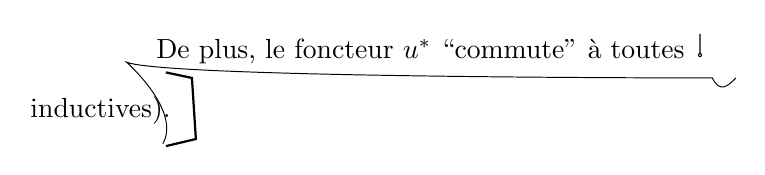
\begin{tikzpicture}[baseline=(ending.base)]
\node[inner sep=1pt] (ending) {inductives).};
\node[anchor=south west,inner sep=2pt] (added) at ([xshift=-3mm,yshift=3mm]ending.north east) {\inserted{\handwritten{De plus, le foncteur $u^{*}$ ``\uline{commute}'' à toutes
\tikz[baseline=-.3ex,scale=.18]{\draw (0,1.5)--(0,.15) .. controls (-.4,-.2) and (.4,-.2) .. (0,.15);}}}};
% One connected thin boundary runs from the close-shaped stroke to below the addition.
\handwritten{\draw[line width=.35pt] ([xshift=-1.4mm,yshift=-2mm]ending.south east) .. controls ([xshift=1mm]ending.east) and ([xshift=-3mm,yshift=1mm]added.south west) .. ([xshift=-3mm,yshift=1mm]added.south west) .. controls ([xshift=2mm,yshift=-1mm]added.south west) and ([xshift=-3mm,yshift=-1mm]added.south east) .. ([yshift=-1mm]added.south east) .. controls ([xshift=1mm,yshift=-3mm]added.south east) and ([xshift=2mm,yshift=-2mm]added.south east) .. ([xshift=3mm,yshift=-1mm]added.south east);
\draw[line width=.8pt] ([xshift=-1mm,yshift=2.7mm]ending.north east)--([xshift=2.3mm,yshift=2mm]ending.north east)--([xshift=2.8mm,yshift=-1.4mm]ending.south east)--([xshift=-1mm,yshift=-2.3mm]ending.south east);}
\end{tikzpicture}
\inserted{\handwritten{
\figure{\begin{tikzpicture}
\node[inner sep=6pt,text width=.88\linewidth,align=left] (topnote) {\tikz[baseline=-.3ex,scale=.18]{\draw (0,1.5)--(0,.15) .. controls (-.4,-.2) and (.4,-.2) .. (0,.15);}les opérations fonctorielles \deleted{\illegible{1}} habituelles faites en termes de telles structures, plus précisément à toutes les opérations qui
\begin{tikzpicture}[baseline=(expr.base)]
\node[inner sep=1pt] (expr) {s'exprime\deleted{nt}\unsure{r}};
\node[anchor=south west,inner sep=1pt] (peuvent) at ([xshift=-1mm,yshift=2mm]expr.north west) {\inserted{peuvent}};
\draw ([xshift=-1mm,yshift=-1mm]expr.south west) .. controls ([xshift=-3mm,yshift=2mm]expr.west) and ([xshift=-1mm,yshift=-1mm]peuvent.south west) .. (peuvent.south east) .. controls ([xshift=1mm]peuvent.south east) .. (peuvent.east);
\end{tikzpicture}
en termes de $\varinjlim$ et de $\varprojlim$ finies: constructions d'objets libres (groupes ou modules libres, p.ex.) engendrés par un objet, produits tensoriels (cf. \S 6 plus bas) etc.};
\draw ([yshift=2mm]topnote.north west) .. controls ([xshift=-2mm]topnote.west) and ([xshift=-1mm]topnote.south west) .. (topnote.south west) -- ([xshift=1mm]topnote.south) -- ([xshift=2mm,yshift=2mm]topnote.south) -- ([yshift=2mm]topnote.south east);
\end{tikzpicture}}}}

\margin{\handwritten{\figure{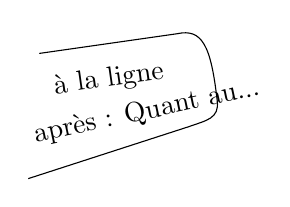
\begin{tikzpicture}[x=1cm,y=1cm]
% margin note slants upward to the right; its two rows are preserved.
\node[anchor=west,rotate=8,inner sep=0pt] (line) at (.05,.62) {à la ligne};
\node[anchor=west,rotate=12,inner sep=0pt] (after) at (-.2,0) {après : Quant au...};
\draw (-.13,1.05)--(1.62,1.3) .. controls (1.94,1.37) and (2.05,1.15) .. (2.13,.45) .. controls (2.16,.22) and (1.99,.2) .. (1.77,.12)--(-.27,-.54);
\end{tikzpicture}}}}
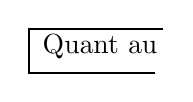
\begin{tikzpicture}[baseline=(quant.base)]
\node[inner sep=2pt] (quant) {Quant au};
\handwritten{\draw[line width=.8pt] (quant.north east)--([xshift=-1mm]quant.north west)--([xshift=-1mm,yshift=-1mm]quant.south west)--([xshift=-1mm,yshift=-1mm]quant.south east);}
\end{tikzpicture}
foncteur image directe
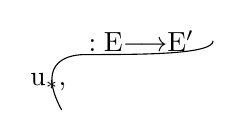
\begin{tikzpicture}[baseline=(direct.base)]
\node[inner sep=1pt] (direct) {$\mathrm{u}_{\handwritten{*}}$,};
\node[anchor=south west,inner sep=1pt] (directmap) at ([xshift=2mm,yshift=2mm]direct.north east) {\inserted{$:\mathrm{E}\handwritten{\longrightarrow}\mathrm{E}'$}};
\handwritten{\draw ([xshift=-1mm,yshift=-2mm]direct.south east) .. controls ([xshift=-4mm,yshift=2mm]direct.east) and ([xshift=-3mm]directmap.south west) .. (directmap.south west) .. controls (directmap.south) and ([xshift=2mm]directmap.south east) .. ([xshift=2mm]directmap.east);}
\end{tikzpicture}
qui commute aux limites projectives, il ``respecte''
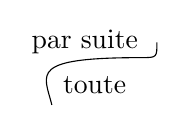
\begin{tikzpicture}[baseline=(toute.base)]
\node[inner sep=1pt] (toute) {toute};
\node[anchor=south west,inner sep=1pt] (suite) at ([xshift=-4mm,yshift=2mm]toute.north west) {\inserted{par suite}};
\handwritten{\draw ([xshift=-1mm,yshift=-1mm]toute.south west) .. controls ([xshift=-2mm]toute.north west) and (suite.south west) .. (suite.south east) .. controls ([xshift=2mm]suite.south east) .. ([xshift=2mm]suite.east);}
\end{tikzpicture}
structure algébrique sur un objet (ou une famille d'objets) de $\mathrm{E}$, définissable en termes de limites projectives
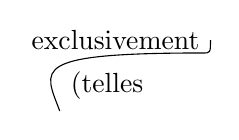
\begin{tikzpicture}[baseline=(telles.base)]
\node[inner sep=1pt] (telles) {(telles};
\node[anchor=south west,inner sep=1pt] (exclusive) at ([xshift=-5mm,yshift=2mm]telles.north west) {\inserted{exclusivement}};
\handwritten{\draw ([xshift=-1mm,yshift=-1mm]telles.south west) .. controls ([xshift=-3mm]telles.north west) and (exclusive.south west) .. (exclusive.south east) .. controls ([xshift=1mm]exclusive.south east) .. ([xshift=1mm]exclusive.east);}
\end{tikzpicture}
les structures de groupe, d'anneau ou de module sur un anneau, \deleted{dans}\inserted{parmi} les exemples précédents). Par
% Both typewriter contours survive in one cell; their order is not established.
\unsure{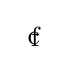
\begin{tikzpicture}[baseline=(contre.base)]\node[inner sep=0pt] (contre) {c};\node[inner sep=0pt] at ([xshift=.15mm,yshift=.12mm]contre.center) {f};\end{tikzpicture}}ontre, le foncteur $\mathrm{u}_{\handwritten{*}}$ n\deleted{e}'est en général pas exact à droite i.e. il ne commute pas en général aux limites inductives finies, et même ne transforme pas en général épimorphisme en épimorphisme\handwritten{\unsure{\begin{tikzpicture}[baseline=-.3ex,x=1ex,y=1ex]
\draw[line width=.6pt] (.3,1.2) .. controls (.16,.77) and (.24,.53) .. (.12,.31) .. controls (-.13,.06) and (.03,-.31) .. (.18,-.26);
\draw[line width=.65pt] (.09,.3) .. controls (.56,.72) and (.47,-.11) .. (.09,.02);
\draw[line width=.6pt] (.4,1.28)--(.48,1.35)--(.52,1.19);
\end{tikzpicture}}} (c'est d'ailleurs
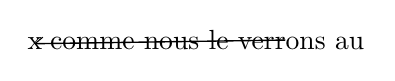
\begin{tikzpicture}[baseline=(comme.base)]
\node[inner sep=1pt] (comme) {\deleted{\unsure{comme} nous le verrons au}};
% An additional cancellation x occupies the preceding blank typewriter cell.
\node[anchor=base east,inner sep=0pt] (cancelx) at ([xshift=-.5mm]comme.base west) {$\mathrm{x}$};
\handwritten{\draw[line width=.5pt] (cancelx.center)--([xshift=.25\linewidth]comme.west);\draw[line width=.4pt] ([xshift=1mm]cancelx.north)--(cancelx.center);}
\end{tikzpicture}
ce défaut d'exactitude du foncteur $\mathrm{u}_{\handwritten{*}}$ qui est \handwritten{à} la source de ces propriétés cohomologiques, qui seront étudiées (du point de vue de l'algèbre homologique commutative) dans l'exposé suivant\handwritten{)}.
\inserted{\handwritten{Par suite, il ne
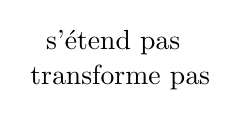
\begin{tikzpicture}[baseline=(trans.base)]
\node[inner sep=1pt] (trans) {\deleted{\unsure{transforme} pas}};
\node[anchor=south west,inner sep=1pt] at ([xshift=2mm,yshift=.5mm]trans.north west) {\inserted{s'étend pas}};
\end{tikzpicture}, en général,
\tikz[baseline=-.3ex,scale=.18]{\draw (0,0)--(.05,1.3) .. controls (-.35,1.65) and (.45,1.65) .. (.05,1.3);}
\figure{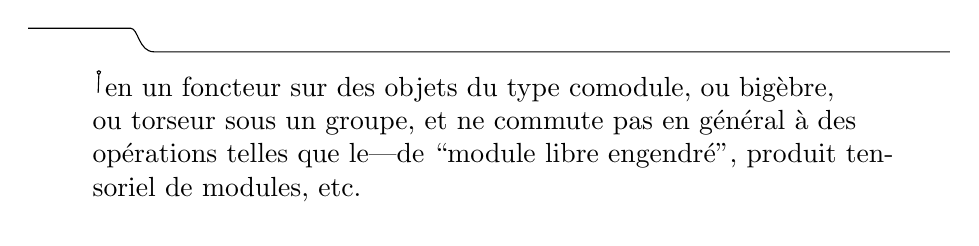
\begin{tikzpicture}
\node[inner sep=6pt,text width=.88\linewidth,align=left] (bottomnote) {\tikz[baseline=-.3ex,scale=.18]{\draw (0,0)--(.05,1.3) .. controls (-.35,1.65) and (.45,1.65) .. (.05,1.3);}en un foncteur sur des objets du type comodule, ou bigèbre, ou torseur sous un groupe\unsure{,} et ne commute pas en général à des opérations telles que \deleted{\unsure{le|de}} ``module libre engendré'', produit tensoriel de modules, etc.};
\draw ([xshift=-6mm,yshift=3mm]bottomnote.north west)--([xshift=7mm,yshift=3mm]bottomnote.north west) .. controls ([xshift=8mm,yshift=3mm]bottomnote.north west) and ([xshift=8mm]bottomnote.north west) .. ([xshift=10mm]bottomnote.north west)--(bottomnote.north east);
\end{tikzpicture}}}}

\deleted{2}\handwritten{3}.1.3. En pratique, lorsqu'on
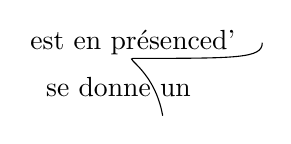
\begin{tikzpicture}[baseline=(presencebase.base)]
\node[inner sep=1pt] (presencebase) {\deleted{se donne} un};
\node[anchor=south west,inner sep=1pt] (presence) at ([xshift=-2mm,yshift=2mm]presencebase.north west) {\inserted{est \inserted{\handwritten{en}} présenced'}};
\handwritten{\draw ([xshift=-4mm,yshift=-2mm]presencebase.south east) .. controls ([xshift=-5mm,yshift=2mm]presencebase.east) and ([xshift=-1mm]presence.south) .. (presence.south) .. controls (presence.south east) and ([xshift=3mm]presence.south east) .. ([xshift=3mm]presence.east);}
\end{tikzpicture}
foncteur $\mathrm{f}:\mathrm{E}\handwritten{\longrightarrow}\mathrm{F}$ d'un $\underline{\mathrm{U}}$-topos dans un autre, il y a lieu d'en expliciter
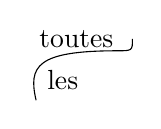
\begin{tikzpicture}[baseline=(les.base)]
\node[inner sep=1pt] (les) {les};
\node[anchor=south west,inner sep=1pt] (toutes) at ([xshift=-1mm,yshift=2mm]les.north west) {\inserted{\handwritten{toutes}}};
\handwritten{\draw ([xshift=-1mm,yshift=-1mm]les.south west) .. controls ([xshift=-2mm]les.north west) and (toutes.south west) .. (toutes.south east) .. controls ([xshift=2mm]toutes.south east) .. ([xshift=2mm]toutes.east);}
\end{tikzpicture}
propri\unsure{
\begin{tikzpicture}[baseline=(propone.base)]\node[inner sep=0pt] (propone) {é};\node[inner sep=0pt] at ([xshift=.1mm]propone.center) {t};\end{tikzpicture}}\unsure{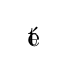
\begin{tikzpicture}[baseline=(proptwo.base)]\node[inner sep=0pt] (proptwo) {t};\node[inner sep=0pt] at ([xshift=.1mm]proptwo.center) {é};\end{tikzpicture}}és d'exactitude, \deleted{y compris et de déterminer s'il admet un foncteur exact} y compris l'existence éventuelle de foncteurs adjoints à gauche ou à droite (cf. la note de bas de page précédente), pour parvenir à une compréhension de la ``nature géométrique'' de $\mathrm{f}$, \deleted{qui} compréhension qui sera généralement un guide indispensable pour
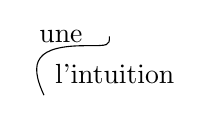
\begin{tikzpicture}[baseline=(intuition.base)]
\node[inner sep=1pt] (intuition) {\deleted{l'}intuition};
\node[anchor=south west,inner sep=1pt] (une) at ([xshift=-2mm,yshift=2mm]intuition.north west) {\inserted{une}};
\handwritten{\draw ([xshift=-1mm,yshift=-1mm]intuition.south west) .. controls ([xshift=-3mm]intuition.north west) and (une.south west) .. (une.south east) .. controls ([xshift=3mm]une.south east) .. ([xshift=3mm]une.east);}
\end{tikzpicture}
géométrique correcte de la situation. Ainsi, s'il s'avère que $\mathrm{f}$ commute aux limites inductives quelconques et aux limites projectives finies, il y a lieu d'écrire $\mathrm{f}$ sous la forme
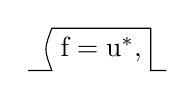
\begin{tikzpicture}[baseline=(n.base)]\node[inner sep=3pt] (n) {$\mathrm{f}=\mathrm{u}^{\handwritten{*}}$,};\handwritten{\draw ([xshift=-3mm]n.south west)--(n.south west) .. controls ([xshift=-1mm]n.west) .. (n.north west)--(n.north east)--(n.south east)--([xshift=2mm]n.south east);}\end{tikzpicture}
où
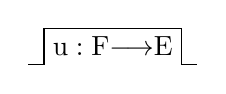
\begin{tikzpicture}[baseline=(n.base)]\node[inner sep=3pt] (n) {$\mathrm{u}:\mathrm{F}\handwritten{\longrightarrow}\mathrm{E}$};\handwritten{\draw ([xshift=-2mm]n.south west)--(n.south west)--(n.north west)--(n.north east)--(n.south east)--([xshift=2mm]n.south east);}\end{tikzpicture}
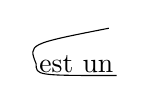
\begin{tikzpicture}[baseline=(n.base)]\node[inner sep=1pt] (n) {est un};\handwritten{\draw ([xshift=-1mm,yshift=3mm]n.north east) .. controls ([xshift=-1mm,yshift=1mm]n.north west) .. (n.west) .. controls (n.south west) .. (n.south east);}\end{tikzpicture}
morphisme de topos, i.e. d'interpréter $\mathrm{f}$ comme un foncteur ``image inverse'' par une ````application continue'' de topos. Lorsque $\mathrm{f}$ commute aux limites projectives quelconques, donc qu'il admet un adjoint à gauche,\deleted{$\mathrm{g}$}\begin{tikzpicture}[baseline=(cancelg.base)]\node[inner sep=0pt] (cancelg) {$\mathrm{x}$};\end{tikzpicture}
% The final separate x is a cancellation impression in the next blank cell.
